\chapter{一些特殊函数的傅里叶变换}
    \section{方波}
        \begin{equation}
            f(t)=E, \quad t\in \left[-\frac{\tau}{2}, \frac{\tau}{2}\right]
            \label{eq: 2.1}
        \end{equation}
        下面求$f(t)$的傅里叶变换结果
        \begin{equation}
            \begin{split}
                \mathscr{F}[f(t)] &= \int_{-\infty}^{\infty}f(t)e^{-i\omega t}\ dt\\
                &= \int_{-\infty}^{\infty}E\ e^{-i\omega t}\ dt\\
                &= -\dfrac{E}{i\omega}e^{-i\omega t}|_{-\frac{\tau}{2}}^{\frac{\tau}{2}}\\
                &= \dfrac{E}{i\omega}(e^{i\omega \frac{\tau}{2}}-e^{-i\omega\frac{\tau}{2}})\\
            \end{split}
            \label{eq: 2.2}
        \end{equation}
        上式利用欧拉定理\myref{eq: 1.2},得到
        \begin{equation}
            \begin{split}
                \mathscr{F}[f(t)] &= \dfrac{E}{i\omega}(e^{i\omega \frac{\tau}{2}}-e^{-i\omega\frac{\tau}{2}})\\
                &= \dfrac{E}{i\omega}(\cos (\omega \dfrac{\tau}{2}) +i \sin(\omega \dfrac{\tau}{2})-\cos (-\omega \dfrac{\tau}{2}) -i \sin(-\omega \dfrac{\tau}{2}))\\
                &= \dfrac{E}{i\omega}(i \sin(\omega \dfrac{\tau}{2}) +i \sin(\omega \dfrac{\tau}{2}))\\
                &= \dfrac{2E}{\omega}\sin\dfrac{\omega\tau}{2}\\
            \end{split}
            \label{eq: 2.3}
        \end{equation}
        图\myref{fig: 2.1}是由Mathematica生成的图像,表示$E = 1, \tau = 1$时的图像
        
        \begin{figure}[h]
            \centering
            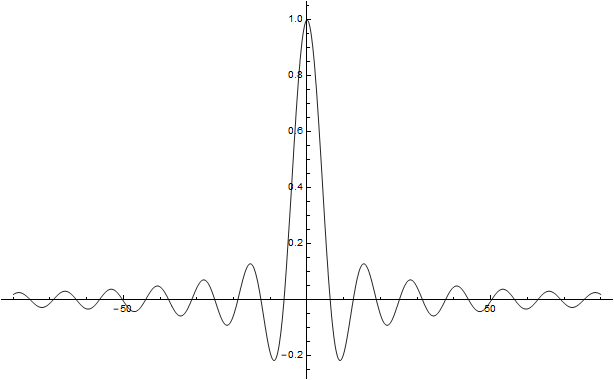
\includegraphics[scale=0.3]{1.png}
            \caption{方波的傅里叶变换}
            \label{fig: 2.1}
        \end{figure}

        应当注意到,这个函数是$\dfrac{\sin x}{x}$的变形,在$x=0$的时候是没有定义的

    \section{$\delta$-函数}

        这是一种广义的函数由一个描述和一个积分式共同定义
        \begin{equation}
            \delta(t) = \left\{
            \begin{aligned}
            \infty & \qquad t=0\\
            0& \qquad else 
            \end{aligned}
            \right.
            \label{eq: 2.4}
        \end{equation}
        并且
        \begin{equation}
            \int_{-\infty}^{\infty}\delta(t)\ dt=\int_{0}^{\epsilon}\dfrac{1}{\epsilon}\ dt=1
            \label{eq: 2.5}
        \end{equation}

        这个函数没办法用图像表示出来,因为它在$t = 0$的时候有一个无穷大的冲激,而在其他地方值为0,就好像用钉子钉墙,一个能量恒定的冲激作用在一个面积很小的点上,而其他的地方则没有能量作用。故这个函数又叫做冲激函数。

        下面证明,$\delta$-函数具有采样性质:
        \begin{equation}
            \int_{-\infty}^{\infty}\delta(t-t_0)f(t)\ dt=f(t_0)
            \label{eq: 2.6}
        \end{equation}

        \begin{proof}
            设$f(t)$是一个在$t_0$处连续的函数
            \begin{equation}
                \int_{-\infty}^{\infty}\delta(t-t_0)f(t)\ dt = \lim_{\epsilon\to 0}\dfrac{1}{\epsilon}\int_{t_0}^{t_0+\epsilon}f(t)\ dt
                \label{eq: 2.7}
            \end{equation}
            
            利用积分中值定理
            \begin{equation}
                \int_{a}^{b}f(x)\ dx = f(\epsilon) (b - a)\qquad a\leq\epsilon\leq b
                \label{eq: 2.8}
            \end{equation}
            可以得到
            \begin{equation}
                \int_{-\infty}^{\infty}\delta(t-t_0)f(t)\ dt = f(\tau)\qquad \tau\in\left[t_0, t_0 + \epsilon\right]
                \label{eq: 2.9}
            \end{equation}
            由于$\epsilon\to 0$,所以
            \begin{equation}
                \int_{-\infty}^{\infty}\delta(t-t_0)f(t)\ dt = f(t_0)
                \label{eq: 2.10}
            \end{equation}
            
            命题得证
        \end{proof}

        证明了这个性质之后,它的傅里叶变换便可以直接得出来:
        \begin{equation}
            \mathscr{F}[\delta(t)]=\int_{-\infty}^{\infty}\delta(t)e^{-i\omega t}\ dt=1
            \label{eq: 2.11}
        \end{equation}


    \section{阶跃函数}
        \begin{definition}
            \begin{equation}
                \epsilon(t)=\left\{
                \begin{aligned}
                0&\qquad t<0\\
                1&\qquad t>0
                \end{aligned}
                \right.
                \label{eq: 2.12}
            \end{equation}
        \end{definition}
        根据定义我们可以知道,阶跃函数的微分即$\delta$-函数

        这里要说明的是,对于阶跃函数的傅里叶变换结果的得出需要使用广义函数的知识,所以这里先给出结果,然后反向证明其正确。
        \begin{equation}
            \mathscr{F}[\epsilon(t)]=\dfrac{1}{i\omega}+\pi\delta(\omega)
            \label{eq: 2.13}
        \end{equation}
        
        为了证明这个式子,需要先证明三个引理:

        \begin{lemma}
            \begin{equation}
                \int \dfrac{1}{x^2 + 1}\ dx=\arctan x+c
                \label{eq: 2.14}
            \end{equation}
        \end{lemma}

        \begin{proof}
            令$\tan y = x$,则
            \begin{equation*}
                \begin{split}
                    \dfrac{dx}{dy}&=\dfrac{d(\tan y)}{dy}\\
                    &=\dfrac{d(\frac{\sin y}{\cos y})}{dy}\\
                    &=\dfrac{\sin^2 y+\cos^2 y}{\cos^2 y}\\
                    &=\tan^2 y+1\\
                    &=x^2+1
                \end{split}
            \end{equation*}
            
            所以
            \begin{equation*}
                \dfrac{dy}{dx}=\dfrac{1}{x^2+1}\Rightarrow\int \dfrac{1}{x^2 + 1}\ dx=\arctan x+c
            \end{equation*}

            证毕
        \end{proof}
        \begin{lemma}
            \begin{equation}
                \int_{0}^{\infty}\sin x e^{-ax}\ dx=\dfrac{1}{a^2+1}
                \label{eq: 2.15}
            \end{equation}
        \end{lemma}
        \begin{proof}
            令
            \begin{equation*}
                I=\int_{0}^{\infty}\sin x e^{-ax}\ dx
            \end{equation*}
            
            则
            \begin{equation*}
                \begin{split}
                    &-I=e^{-ax}\cos x\bigg|_{0}^{\infty}+\int_{0}^{\infty}a\cos x e^{-ax}\ dx\\
                    &\Rightarrow -I=-1+a\int_{0}^{\infty}\cos x e^{-ax}\ dx\\
                    &\Rightarrow \dfrac{1-I}{a}=\int_{0}^{\infty} e^{-ax}\ d\sin x\\
                    &\Rightarrow \dfrac{1-I}{a}=e^{-ax}\sin x\bigg|_{0}^{\infty}+\int_{0}^{\infty} a\sin x e^{-ax}\ dx\\
                    &\Rightarrow \dfrac{1-I}{a}=0+aI\\
                    &\Rightarrow I=\dfrac{1}{a^2+1}\\
                \end{split}
            \end{equation*}

            证毕
        \end{proof}

        \begin{lemma}{Dirichlet积分}
            \begin{equation}
                \int_{0}^{\infty}\dfrac{\sin x}{x}\ dx=\dfrac{\pi}{2}
                \label{eq: 2.16}
            \end{equation}
        \end{lemma}

        我们知道,这个函数在零点是无意义的,而且它的积分是一个反常积分,只有无穷级数形式,没有解析表达式,这就导致求它的积分需要特殊的方法

        下面分别用\emph{多重积分}和\emph{费曼技巧}两种证明方法对该结论进行证明

        \begin{proof}
            令
            \begin{equation*}
                \begin{split}
                    I_1=\int_{0}^{\infty}\int_{0}^{\infty}e^{-xy}\sin y\ dxdy\\
                    I_2=\int_{0}^{\infty}\int_{0}^{\infty}e^{-xy}\sin y\ dydx
                \end{split}
            \end{equation*}

            由于这两个二重积分仅仅是积分次序不用,所以很显然有$I_1=I_2$,并且由$I_1$得到:
            \begin{equation*}
                \begin{split}
                    I_1&=\int_{0}^{\infty}\sin y(\int_{0}^{\infty}e^{-xy}\ dx)dy\\
                    &=\int_{0}^{\infty}\sin y(-\frac{1}{y}e^{-xy})\big|_0^\infty dy\\
                    &=\int_{0}^{\infty}\dfrac{\sin y}{y} dy\\
                \end{split}
            \end{equation*}

            由\myref{eq: 2.14}和\myref{eq: 2.15}可以得到
            \begin{equation*}
                I_2=\int_{0}^{\infty}\dfrac{1}{x^2+1}\ dx=\arctan x\bigg|_{0}^{\infty}=\dfrac{\pi}{2}\tag*{}
            \end{equation*}

            由$I_1=I_2$得到结果,证毕.
        \end{proof}

        下面的方法被称为\emph{费曼技巧},这是一种求定积分的有效方法,由理查德·费曼使用并推广,简要来说叫做“积分内取微分”

        \begin{proof}
            令
            \begin{equation*}
                I(a)=\int_{0}^{\infty}\dfrac{\sin x}{x}e^{-ax}\ dx
            \end{equation*}

            将该函数对变量$a$取微分
            \begin{equation*}
                \begin{split}
                    &\dfrac{dI(a)}{da}=\int_{0}^{\infty}-x\dfrac{\sin x}{x}e^{-ax}\ dx\\
                    &\Rightarrow \dfrac{dI(a)}{da}=-\int_{0}^{\infty}\sin x e^{-ax}\ dx=-\dfrac{1}{a^2+1}
                \end{split}
            \end{equation*}

            对上述结果再取定积分
            \begin{equation*}
                \begin{split}
                    &\int_{0}^{\infty}-\dfrac{1}{a^2+1}\ dx=I(\infty)-I(0)\\
                    &\Rightarrow -\dfrac{\pi}{2}=-I(0)\\
                    &\Rightarrow\int_{0}^{\infty}\dfrac{\sin x}{x}\ dx=\dfrac{\pi}{2}
                \end{split}
            \end{equation*}

            证毕
        \end{proof}

        证明了上面的三个引理之后,可以来证明结论了:
        \begin{proof}
            假如命题正确,则有
            \begin{equation*}
                \begin{split}
                    \epsilon(t)&=\mathscr{F}^{-1}[\dfrac{1}{i\omega}+\pi\delta(\omega)]\\
                    &=\dfrac{1}{2\pi}\int_{-\infty}^{\infty}[\dfrac{1}{i\omega}+\pi\delta(\omega)] e^{i\omega t} d\omega\\
                    &=\dfrac{1}{2\pi}\int_{-\infty}^{\infty}\dfrac{1}{i\omega} e^{i\omega t} d\omega+\dfrac{1}{2\pi}\int_{-\infty}^{\infty}\pi\delta(\omega) e^{i\omega t} d\omega\\
                    &=\dfrac{1}{2\pi}\int_{-\infty}^{\infty}\dfrac{1}{i\omega} (\cos \omega t +i \sin\omega t)\ d\omega+\dfrac{1}{2}\\
                    &=\dfrac{1}{\pi}\int_{0}^{\infty}\dfrac{\sin\omega t}{\omega}\ d\omega+\dfrac{1}{2}\\
                \end{split}
            \end{equation*}

            由\myref{eq: 2.16}我们知道,$\int_{0}^{\infty}\dfrac{\sin\omega}{\omega}\ d\omega=\dfrac{\pi}{2}$,由于$t\omega\sim\omega$,故存在下列关系
            \begin{equation*}
                \int_{0}^{\infty}\dfrac{\sin\omega t}{\omega}\ d\omega=\left\{\begin{aligned}
                -\frac{\pi}{2}&\qquad t<0\\
                0&\qquad t=0\\
                \dfrac{\pi}{2}&\qquad t>0
                \end{aligned}\right.
            \end{equation*}

            故
            \begin{equation*}
                \epsilon(t)=\left\{\begin{aligned}
                \dfrac 1 2 + \dfrac \pi 2(-\frac{\pi}{2})&\qquad t<0\\
                \dfrac 1 2 + \dfrac \pi 2(\dfrac{\pi}{2})&\qquad t>0
                \end{aligned}\right.\Rightarrow\left\{\begin{aligned}
                0&\qquad t<0\\
                1&\qquad t>0
                \end{aligned}\right.
            \end{equation*}

            这正是阶跃函数,所以命题成立
        \end{proof}
    \section{1}
        以上面这种先入为主的方式,我们再来捡几个傅里叶变换对:
        \begin{equation}
            \mathscr{F}[1]=2\pi\delta(\omega)
            \label{eq: 2.17}
        \end{equation}
        \begin{proof}
            \begin{equation*}
                \mathscr{F}^{-1}[2\pi\delta(\omega)]=\dfrac{1}{2\pi}\int_{-\infty}^{\infty}2\pi\delta(\omega)e^{i\omega t}\ d\omega=1\tag*{}
            \end{equation*}
            证毕
        \end{proof}

        结合\myref{eq: 2.11},发现这其实是两对傅里叶变换对
    \section{指数函数}
        \begin{equation}
            \mathscr{F}[e^{i\omega_0 t}]=2\pi\delta(\omega-\omega_0)
            \label{eq: 2.18}
        \end{equation}
        \begin{proof}
            \begin{equation*}
                \begin{split}
                    &\mathscr{F}^{-1}[2\pi\delta(\omega-\omega_0)]=\dfrac{1}{2\pi}\int_{-\infty}^{\infty}2\pi\delta(\omega-\omega_0)e^{i\omega t}\ d\omega\\
                    &=\int_{-\infty}^{\infty}\delta(\omega-\omega_0)e^{i(\omega-\omega_0) t}\ d(\omega-\omega_0)\cdot e^{i\omega_0 t}\\
                    &=e^{i\omega_0 t}
                \end{split}
            \end{equation*}
            证毕
        \end{proof}
    \section{正弦函数}
        有了以上的几个傅里叶变换对之后,就可以很容易地求出其他的傅里叶变换,比如正弦函数:
        \begin{equation}
            \begin{split}
                \mathscr{F}[\sin \omega_0t]&=\int_{-\infty}^{\infty}\sin(\omega_0t)e^{-i\omega t}\ dt\\
                &=\int_{-\infty}^{\infty}\dfrac{e^{i\omega_0t}-e^{-i\omega_0t}}{2i}e^{-i\omega t}\ dt\\
                &=\dfrac{1}{2i}\int_{-\infty}^{\infty}(e^{i\omega_0t}-e^{-i\omega_0t})e^{-i\omega t}\ dt\\
                &=\dfrac{1}{2i}\int_{-\infty}^{\infty}(e^{-i(\omega - \omega_0)t}-e^{-i(\omega  + \omega_0)t})\ dt\\
                &=\dfrac{1}{2i}(\mathscr{F}[e^{i\omega_0 t}]-\mathscr{F}[e^{-i\omega_0 t}])\\
                &=\dfrac{1}{2i}(2\pi\delta(\omega-\omega_0)-2\pi\delta(\omega+\omega_0))\\
                &=i\pi(\delta(\omega+\omega_0)-\delta(\omega-\omega_0))\\
            \end{split}
            \label{eq: 2.19}
        \end{equation}
    \section{指数衰减函数}
        \begin{equation}
            f(t)=\left\{\begin{aligned}
            0&\qquad t<0\\
            e^{-\beta t}&\qquad t\geq0
            \end{aligned}
            \right.(\beta>0)
            \label{eq: 2.20}
        \end{equation}

        它的傅里叶变换不需要广义函数加持
        \begin{equation}
            \begin{split}
                \mathscr{F}[f(t)]&= \int_{-\infty}^{\infty}f(t)e^{-i\omega t}\ dt\\
                &= \int_{0}^{\infty}e^{-\beta t}e^{-i\omega t}\ dt\\
                &= \int_{0}^{\infty}e^{-(\beta + i\omega) t}\ dt\\
                &= \dfrac{1}{\beta+i\omega}=\dfrac{\beta-i\omega}{\beta^2+\omega^2}
            \end{split}
            \label{eq: 2.21}
        \end{equation}
    \section{一些思考}
        从上面的结果可以看到,$\delta$-函数可以用来组成所有的非周期函数的傅里叶变换,这一点非常有用

        下面来总结一下刚刚得到的几个傅里叶变换对
        
        \[
            \begin{array}{|c|c|}
                \hline
                \text{时域} & \text{频域}\\ \hline
                E & \frac{2E}{\omega}\sin\frac{\omega\tau}{2}\\ \hline
                \delta(t) & 1\\ \hline
                \epsilon(t) & \frac{1}{i\omega}+\pi\delta(\omega)\\ \hline
                1 & 2\pi\delta(\omega)\\ \hline
                e^{i\omega_0 t} & 2\pi\delta(\omega-\omega_0)\\ \hline
                \sin \omega_0t & i\pi(\delta(\omega+\omega_0)-\delta(\omega-\omega_0))\\ \hline
                e^{-\beta t}\quad t\geq0 & \dfrac{\beta-i\omega}{\beta^2+\omega^2}\\ \hline
            \end{array}
        \]